\begin{figure*}
\centering
\begin{subfigure}[b]{0.48\textwidth}
    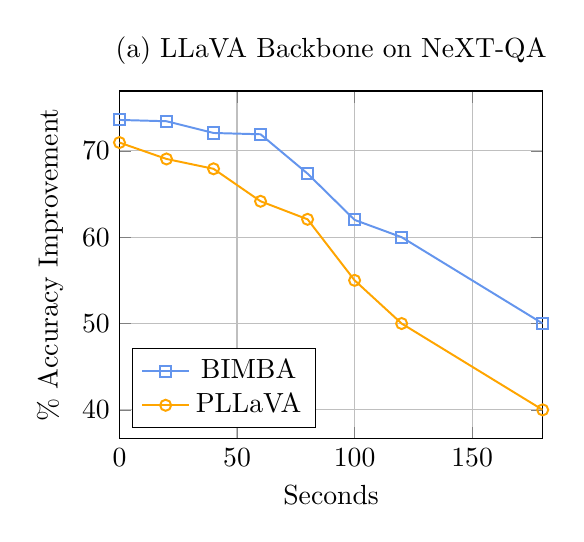
\begin{tikzpicture}
    \begin{axis}[
        % width=12cm, 
        height=6cm,
        xlabel={Seconds},
        ylabel={\% Accuracy Improvement},
        title={(a) LLaVA Backbone on NeXT-QA},
        xmin=0, xmax=180,
        % ymin=0, ymax=30,
        % xtick={5000, 10000, 15000, 20000,25000,30000, 35000},
        % xticklabels={5K, 10K, 15K, 20K, 25K,30K, 35K},
        %ytick={60, 62, 64, 66, 68, 70, 72, 74},
        legend pos=south west,
        grid=both,
        scaled ticks = false,
        scaled x ticks = false,
    ]

    
    %BIMBA Data
    \addplot[line width=.25mm, color=CornflowerBlue, mark=square, mark size=2pt]
coordinates {
(0, 73.58)
(20, 73.43)
(40, 72.07)
(60, 71.92)
(80, 67.36)
(100, 62.0)
(120, 60.0)
(180, 50.0)
};
    \addlegendentry{BIMBA}

    \addplot[line width=.25mm, color=Orange, mark=o, mark size=2pt]
coordinates {
(0, 70.96)
(20, 69.06)
(40, 67.92)
(60, 64.16)
(80, 62.07)
(100, 55.0)
(120, 50.0)
(180, 40.0)
};
    \addlegendentry{PLLaVA}

    \end{axis}
    \end{tikzpicture}
% \caption{Figure 1}
\end{subfigure}
\hfill
\begin{subfigure}[b]{0.48\textwidth}
    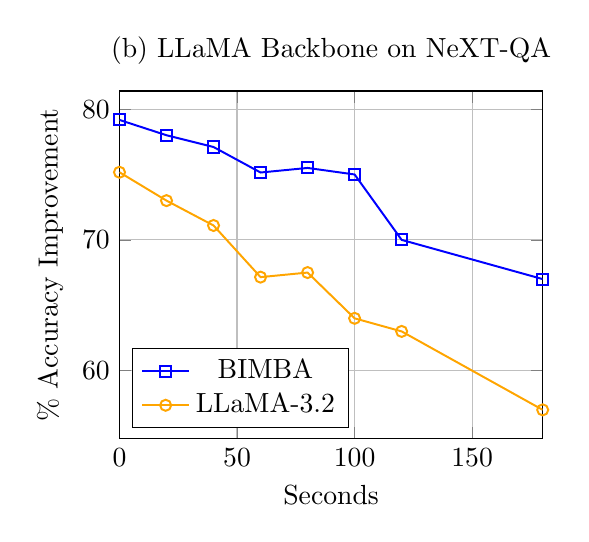
\begin{tikzpicture}
    \begin{axis}[
        % width=12cm, 
        height=6cm,
        xlabel={Seconds},
        ylabel={\% Accuracy Improvement},
        title={(b) LLaMA Backbone on NeXT-QA},
        xmin=0, xmax=180,
        % ymin=0, ymax=20,
        % xtick={5000, 10000, 15000, 20000,25000,30000, 35000},
        % xticklabels={5K, 10K, 15K, 20K, 25K,30K, 35K},
        % ytick={60, 62, 64, 66, 68, 70, 72, 74},
        legend pos=south west,
        grid=both,
        scaled ticks = false,
        scaled x ticks = false,
    ]
    % BIMBA Data


    \addplot[line width=.25mm, color=Blue, mark=square, mark size=2pt]
    coordinates {
(0,79.17)
(20, 78.0)
(40,77.1)
(60, 75.15)
(80, 75.5)
(100, 75.0)
(120, 70.0)
(180, 67.0)
};
    \addlegendentry{BIMBA}

        \addplot[line width=.25mm, color=Orange, mark=o, mark size=2pt]
    coordinates {
(0,75.17)
(20, 73.0)
(40,71.1)
(60, 67.15)
(80, 67.5)
(100, 64.0)
(120, 63.0)
(180, 57.0)
};
    \addlegendentry{LLaMA-3.2}
    
    \end{axis}
    \end{tikzpicture}
    % \caption{Figure 2}
\end{subfigure}
\caption{Performance Using LLaVA Backbone}
\label{fig:performance llava}
\end{figure*}



